\documentclass[crop,tikz]{standalone}
\usetikzlibrary{backgrounds}
\colorlet{blue}{cyan}
\tikzset{
  inverted/.style = {
    color=white,
    background rectangle/.style={fill},
    show background rectangle
  }
}

\usepackage{amsmath}
\usepackage[european,americaninductors]{circuitikz}
\usetikzlibrary{patterns}
\tikzset{>=latex}
\colorlet{green}{green}
\colorlet{red}{red!80!white}
\colorlet{lightgray}{gray!50!white}
\colorlet{darkgray}{gray!80!white}

\begin{document}
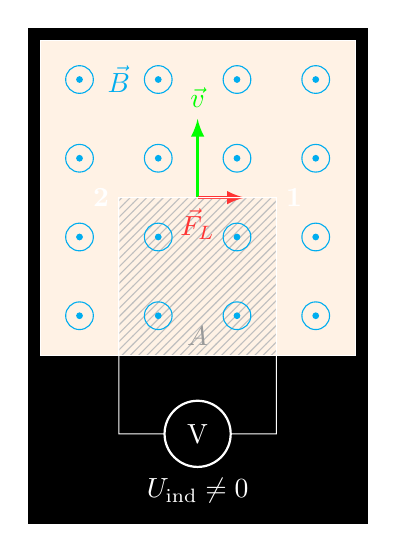
\begin{tikzpicture}[inverted,inverted]
  \draw[fill=orange!10] (-4,-4) rectangle ++ (4,4);
  \draw[pattern=north east lines,pattern color=lightgray] (-3,-4) rectangle ++ (2,2);
  \node[darkgray,above] at (-2,-4) {$A$};
  % magnetic field
  \foreach \X in {-3.5,...,-0.5} {
    \foreach \Y in {-3.5,...,-0.5} {
      \draw[fill,blue] (\X,\Y) circle (1pt);
      \draw[blue] (\X,\Y) circle (5pt);
    }    
  }
  \node[blue] at (-3,-0.5) {$\vec{B}$};
  % velocity
  \draw[very thick,green,->] (-2,-2) coordinate (v) -- ++(0,1) node[above] {$\vec{v}$};
  % Lorentz force
  \draw[very thick,red,->] (v) node[below] {$\vec{F}_L$} -- ++(0.6,0);
  % circuit
  \draw[] (-3,-2) node [left] {\textbf{2}}
    to[] ++(2,0) node [right] {\textbf{1}}
    to[] ++(0,-3)
    to[rmeter={$U_{\text{ind}}\neq 0$},t=V] ++(-2,0)
    to[] ++(0,3);
\end{tikzpicture}
\end{document}
